\chapter{Nesting}
\label{nesting_chap}

ARW provides the capability to concentrate the area of importance of a simulation
via nesting options. 
ARW supports horizontal nesting that allows resolution to be
focused over a region of interest by introducing an additional grid (or
grids) into the simulation.  This subdomain with increased horizontal resolution is completely
contained within the parent domain. Vertical refinement options are also 
available, where a child domain may have a different vertical structure than
the parent domain. The child and parent domains always extend from the lower model surface
through to the upper model lid. In this way, the vertical capabilty is more accurately referred
to as a "refinement" as opposed to "nesting". In practice, both of these terms will be used 
interchangeably when referring to a child domain that has enhanced vertical resolution 
compared to the parent domain.

As with all domains within ARW, the horizontally or vertically nested grids (child domains, 
fine-grid domains) are rectangular
and are aligned with the parent (coarser) grid within which they are
nested.  
The horizontal nested grids allow any integer spatial
($\Delta x_{coarse}/\Delta x_{fine}$) 
and temporal refinements of the
parent grid (the spatial and temporal refinements are usually,
but not necessarily the same).  
The vertical refinement capability offers two options: either an integer factor of the
number of levels in the parent to define the child domain's vertical structure (for example, 
a doubling or tripling of the vertical resolution), or a completely independent set of 
vertical levels prescribed for the parent and the child domain.
The horizontal nesting capability is in many ways similar to the
implementations provided in other mesoscale and cloudscale models (e.g. MM5,
ARPS, COAMPS). The vertical refinement options are described in 
\citet{mahalovmoustaoui09} and \citet{daniels16}.

ARW's nesting
infrastruture computes nested
simulations efficiently on parallel distributed-memory computer systems,
which includes support for moving nested grids.
The WRF Software Framework, described in
\citet{michalak04}, makes these capabilities possible.  In this chapter we
describe the various horizontal and vertical nesting options available in ARW and the 
numerical coupling between the grids.

\section {Horizontal Nesting Options}

%
% 1-way vs 2-way
%
\begin{figure} 
 \centering
  \includegraphics *[width=4.5in]{figures/12way_v4.pdf}
  \caption{\label{figure:12way} 1-way (parent provides boundary data to child) and 
   2-way (parent provides boundary data to child, then child feeds information back to
   the parent) nesting options in ARW.}
\end{figure}

\subsubsection{1-Way and 2-Way Grid Nesting}

Nested grid simulations can be produced using either 1-way
nesting or 2-way nesting as outlined in Fig. \ref{figure:12way}.  The
1-way and 2-way nesting options refer to how a coarse grid and the
fine grid interact.  In both the 1-way and 2-way simulation modes, the
fine grid boundary conditions (i.e., the lateral boundaries) are interpolated
from the coarse grid forecast.  In a 1-way nest, this is the only
information exchange between the grids (from the coarse grid to the fine grid).
Hence, the name {\em 1-way nesting}.  In the 2-way nest integration, the
fine grid solution replaces the coarse grid solution for coarse
grid points that lie inside the fine grid.  This information exchange
between the grids is now in both directions (coarse-to-fine for the 
fine-grid lateral boundary computation and
fine-to-coarse during the feedback at each coarse-grid time step).  
Hence, the name {\em 2-way nesting}.

The 1-way nest set-up may be run in one of two different methods.  One
option is to produce the nested simulation as two separate ARW simulations
as described in the leftmost box in Fig. \ref{figure:12way}.  In this mode,
the coarse grid is integrated first and the coarse grid forecast is completed.  
Output from the coarse grid
integration is then processed to provide boundary conditions for
the nested run (usually at a much lower temporal frequency than the
coarse grid time step), and this is followed by the complete time
integration of fine (nested) grid.  Hence, this 1-way option is equivalent
to running two separate simulations with a processing step in between.  Also with
separate grid simulations, an intermediate re-analysis (such as
via WRFDA, see Section \ref{var_chap}) can be included.

The second 1-way option (lockstep with no feedback), depicted in the
middle box in Fig. \ref{figure:12way}, is run as a traditional
simulation with two (or more) grids integrating concurrently, except with
the feedback runtime option shut off.  This option provides lateral boundary
conditions to the fine grid at each coarse grid time step, which
is an advantage of the concurrent 1-way method (no feedback).


\subsubsection{Fine Grid Initialization Options}

ARW supports several strategies to horizontally refine a coarse-grid 
simulation with the introduction of a nested grid.  When using concurrent 1-way and
2-way nesting, several options for initializing the fine grid
are provided.
\begin{itemize}\setlength{\parskip}{-4pt}
\item All of the fine grid variables (both meteorological and 
terrestrial) can be interpolated from the coarse grid (useful
when a fine grid starts later in the coarse-grid forecast).
\item All of the fine grid variables can be input from an external file
which has high-resolution information for both the meteorological 
and the terrestrial fields (a standard set-up when the fine-grid 
terrestrial fields are expected to impact the forecast).
\item The fine grid can have some of the variables initialized with a
high-resolution external data set, while other variables are
interpolated from the coarse grid (for example this would permit 
the improved analysis from the WRFDA initialization of the
coarse grid's meteorological fields to remain consistent with the fine grid).
This option allows the fine grid to start later in the coarse-grid's
forecast, but with the advantage of higher-resolution static fields.
\item For a moving nest, external orography and landuse files may be used 
to update the fine-grid domain as it moves over land.
\end{itemize}

\noindent These fine grid initialization settings are user specified at
run-time, and ARW allows nested grids to instantiate and cease during any
time that the fine grid's parent is still integrating. While cost savings are
evident when starting the fine-grid domain at a later time, that advantage 
must be weighed against the impact of relatively coarse and inconsistent
fields for both masked and meteorological variables on the fine grid.
%
% nest grids, some OK, some illegal
%
\begin{figure} 
 \centering
  \includegraphics *[width=6.0in]{figures/nest_domains.pdf}
  \caption{\label{figure:nest_domains}Various nest configurations for multiple grids.  (a)
   Telescoping nests. (b) Nests at the same level with respect to a parent grid.
   (c) Overlapping grids: not allowed with feedback activated.  
   (d) Inner-most grid has more than one parent grid: not allowed}
\end{figure}


\subsubsection{Possible Grid Configurations}

A simulation involves one outer grid and may contain multiple
inner nested grids.  In ARW, each nested region is entirely
contained within 
a single coarser grid, referred to as the {\em parent}
grid.  The finer, nested grids are referred to as {\em child} grids.
Using this terminology, children are also parents when multiple levels
of nesting are used.  The fine grids may be telescoped to any depth (i.e., 
a
parent grid may contain one or more child grids, each of which in turn
may successively contain one or more child grids; Fig.
\ref{figure:nest_domains}a), and several fine grids may share the
same parent at the same level of nesting (Fig.
\ref{figure:nest_domains}b).  
Any valid fine grid may either be a static domain or it may be a moving nest
(with either prescribed incremental shifts or with automatic moves
via a vortex following algorithm, such as tracking the minimum of the 500 mb height).  
ARW does not permit overlapping
grids, where a coarse grid point is contained within more than a
single child grid (i.e., both of which are at the same nest level with respect
to the parent; Fig. \ref{figure:nest_domains}c).  In addition, no grid can have
more than a single parent (Fig. \ref{figure:nest_domains}d).  For global domains, a
fine grid domain cannot cross the periodic lateral boundary of the parent domain
(for example, a global domain may not have a nested tropical channel at the 
equator that uses periodic east-west boundaries in the nest.)

For both 1-way and 2-way nested grid simulations, the ratio of the
parent horizontal grid distance to the child horizontal grid distance
(the spatial refinement ratio) must be an integer.  For 2-way and concurrent 1-way
nesting, this is also true for
the time steps (the temporal refinement ratio).  The model does allow
the time step refinement ratio to differ from the spatial refinement
ratio.  Also, nested grids on the same level (i.e., children who have the
same parent) may have different spatial and temporal refinement ratios.  For example,
in Fig. \ref{figure:nest_domains}b, the horizontal grid resolution for 
domain 1 could be 90 km, for
domain 2 could be 45 km, and for domain 3 could be 30 km.

\subsubsection{Moving Nests}

The moving nest capabilities in ARW are simply extensions to the 
suite of nesting options.  All descriptions covering the 
specifics for the fine-grid
domains (initialization, feedback, configurations, staggering,
lateral boundaries, etc.) apply also to moving nests.  In
general, all nests
in an ARW forecast are eligible to be moving nests.  ARW
provides two methods to have nests move during the model
integration: specified and automatic.
For both types of moving nests,
multiple levels of domains may move.  

For a specified move, the timing of a nest move and the extent
of each lateral move is defined entirely by the user through
the namelist. This manual process is tedious and cumbersome, and is 
rarely used in practice. This capability was required to eventually
develop a fully functioning moving nest capability that automatically 
tracks a cyclone.  

For the
automatically moving nest, the fine grid is initialized to cover
a well-defined vortex, and the nest moves to maintain this vortex
in the center of the fine grid. The fine grid follows a height 
minimum, and is constrained so as to not too closely approach 
the parent boundary. This option provides a substantial cost savings
when the area of horizontal refinement is reduced in 
size to cover only the physical extent of a cyclone, and not the 
much larger domain necessary to contain a moving system.
Most of the 
instances where a moving nest is utilized are during tropical
cyclone tracking via the automatic vortex following technique,
where the inner-most nest drives the moving domains.

After a nested domain has moved a parent grid-cell distance,
the majority of the fine-grid data in the domain is still valid.  The
data that is not along the outer row or column of the nested
domain is shifted to the new location in that domain: not interpolated
from the parent domain.
Once a domain moves, the data in the outer
row or column falls into two categories: discarded data on the
trailing edge, and horizontally interpolated data on the
leading edge in the direction of the nest move. 
Only the topography elevation and the landuse categories are elegible
to be input from high-resolution files instead of an interpolation
from the parent domain.

\section{Staggering and Feedback}

ARW uses an Arakawa-C grid staggering.  As shown in Fig.
\ref{figure:cg_fg}, the $u$ and $v$ components 
of horizontal velocity are normal to the respective faces of the 
grid cell, and the mass/thermodynamic/scalar/chemistry variables are located 
in the center of the cell.   

%
% Figure colorful single-grid u,v,t stagger
%
\begin{figure}
  \centering
  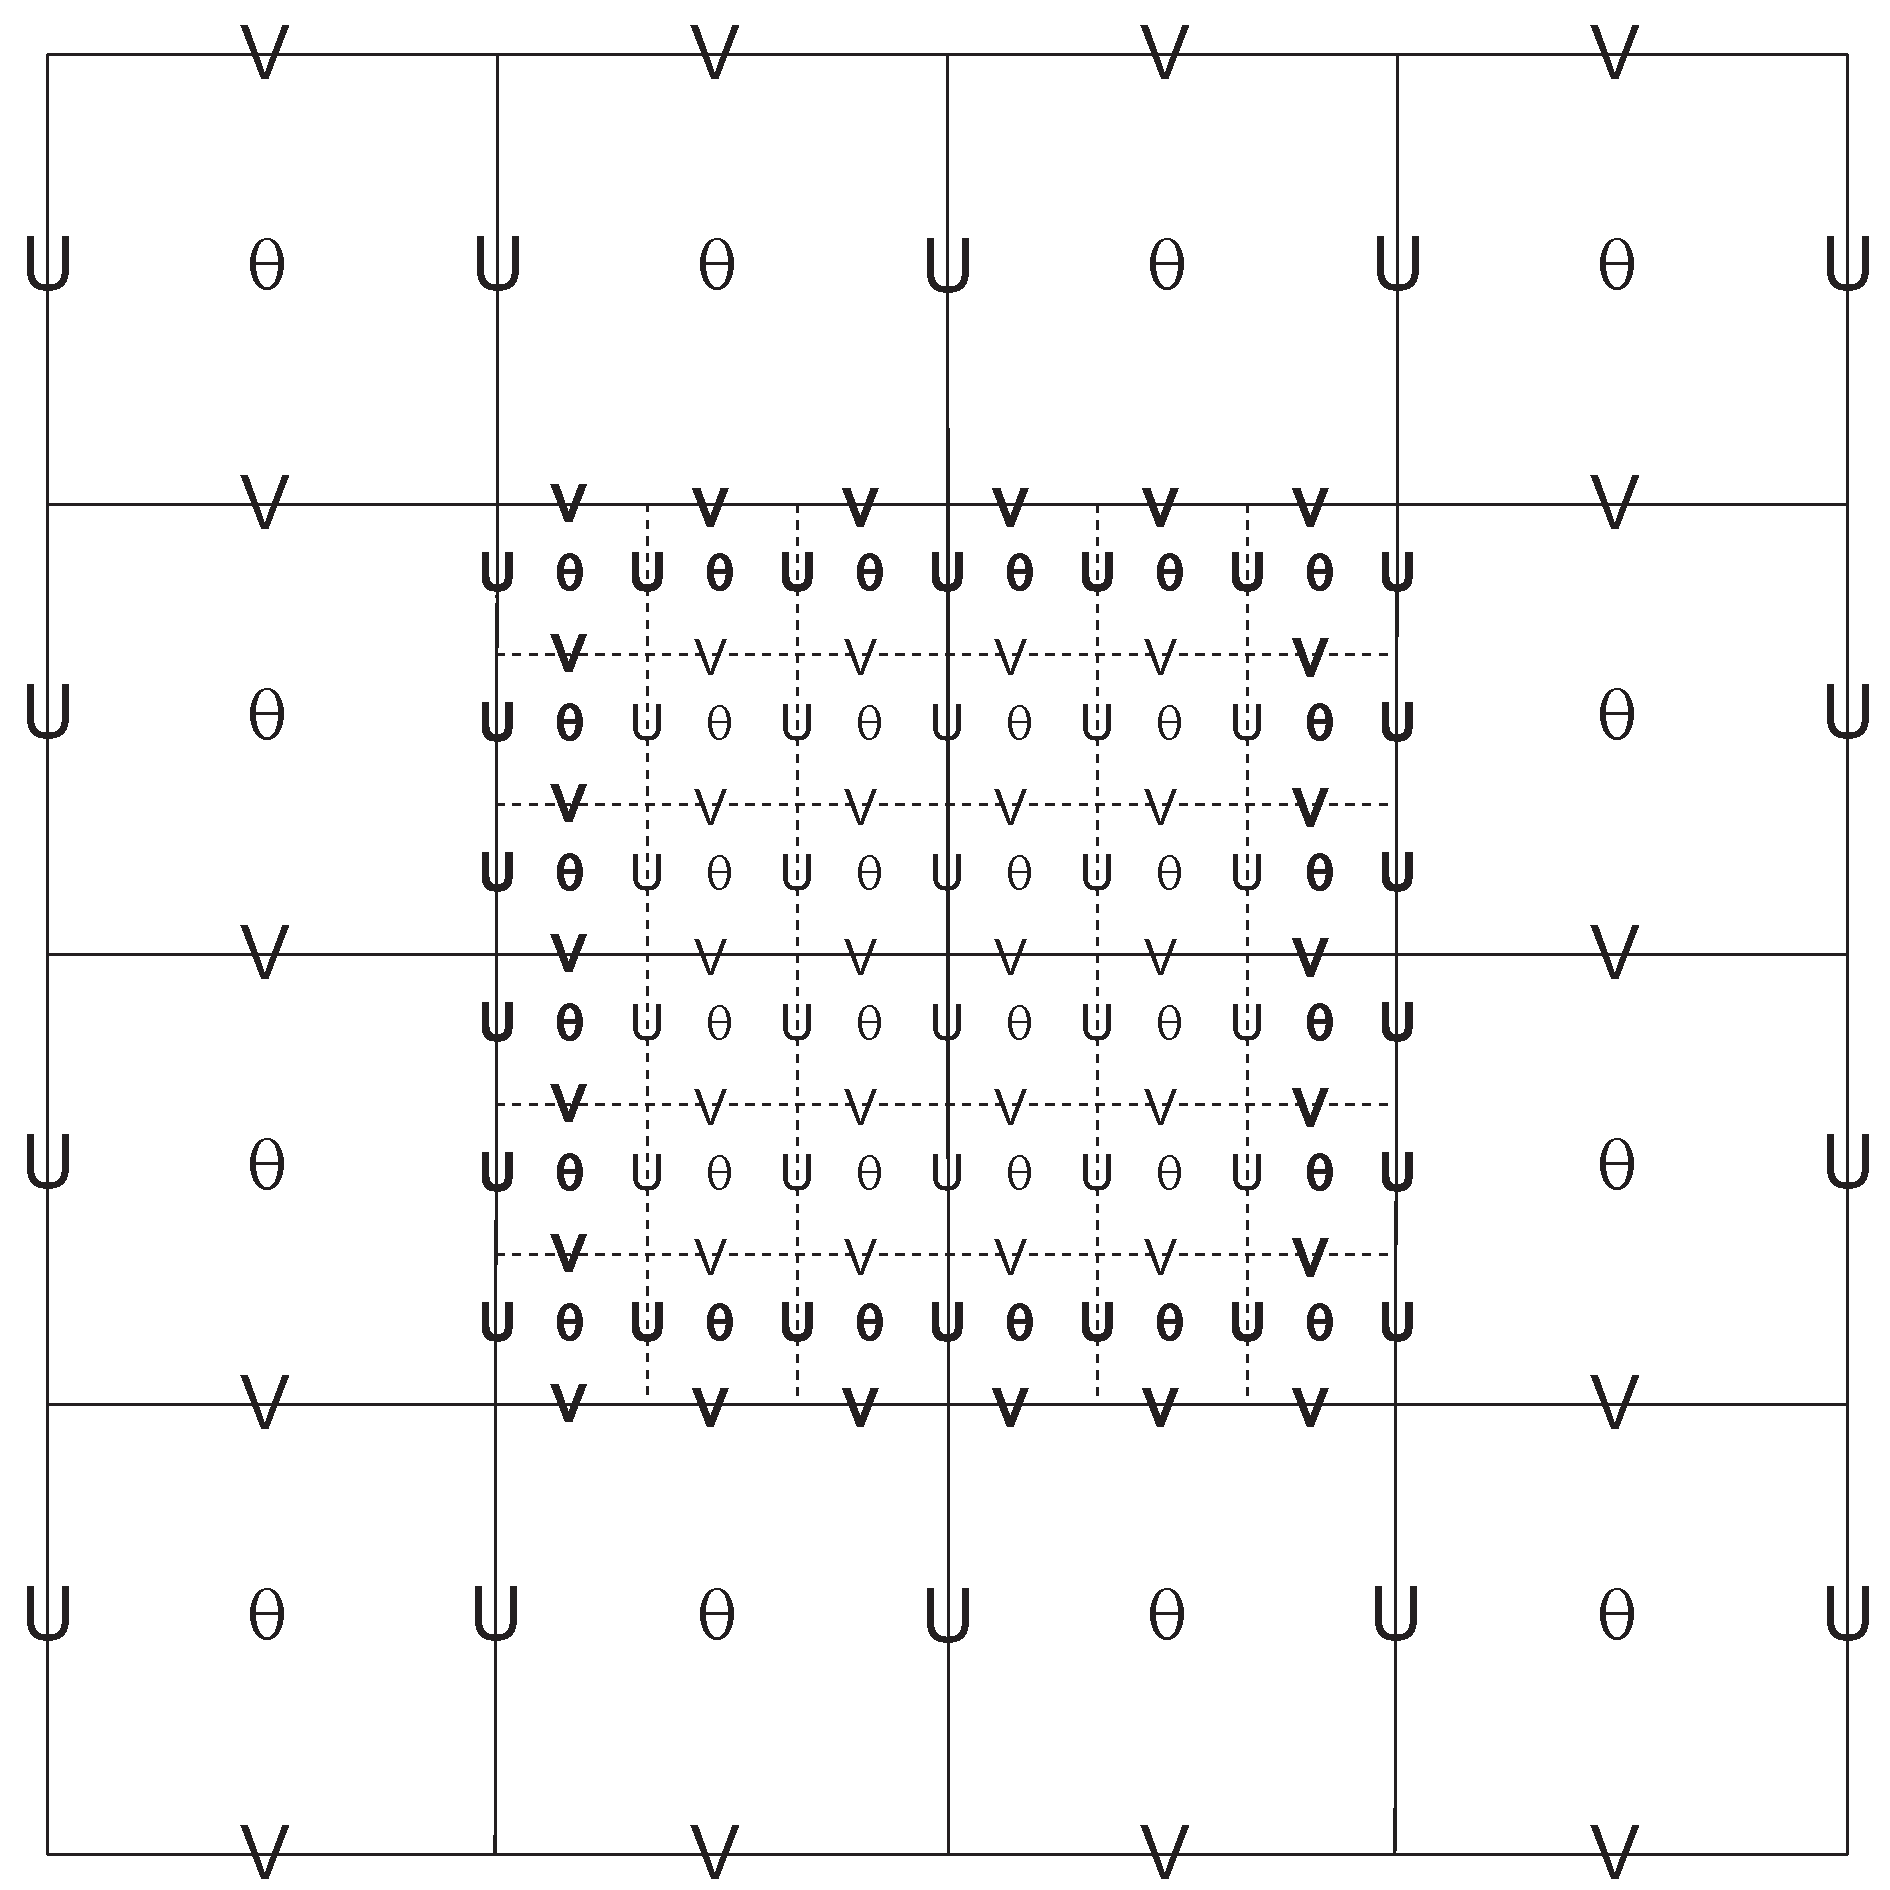
\includegraphics[width=4in]{figures/cg_fg.pdf}
  \caption{\label{figure:cg_fg}
Arakawa-C grid staggering for a portion of a parent domain and an
imbedded nest domain with a 3:1 grid size ratio.  The solid lines
denote coarse grid cell boundaries, and the dashed lines are the
boundaries for each fine grid cell.  The horizontal components of
velocity (``U'' and ``V'') are defined along the normal cell face, and
the thermodynamic variables (``$\theta$'') are defined at the center of
the grid cell (each square).  The bold typeface variables along the
interface between the coarse and the fine grid define the locations
where the specified lateral boundaries for the nest are in
effect.  } \end{figure}

The variable staggering has an additional column 
of $u$ in the x-direction and an additional row of $v$ in the y-direction
because the normal velocity points define the grid boundaries.
The horizontal momentum components reflect an average across each 
cell-face, while each mass/thermodynamic/scalar/chemistry variable
is the representative mean value throughout the cell.  
Feedback is handled to preserve these mean values: the mass/thermodynamic/scalar/chemistry
fields are fed back with an average from within the entire 
coarse grid point (Fig. \ref{figure:cg_fg}), and the horizontal momentum variables are
averaged along their respective normal coarse grid cell faces.

The horizontal interpolation (to instantiate a grid and to provide 
time-dependent lateral boundaries) does not conserve mass.  The 
feedback mechanism, for most of the unmasked fields, uses cell 
averages (for mass/thermodynamic/scalar/chemistry quantities) and cell-face 
averages for the horizontal momentum fields.


The staggering defines the way that the fine grid is situated 
on top of the coarse grid.  For all odd ratios there is a coincident 
point for each variable: a location that has the coarse grid 
and the fine grid at the same physical point.  The location of 
this point depends on the variable. 
In each of the 
coarse-grid cells with an odd ratio, the middle fine-grid cell
is the coincident point with the coarse grid for all of the 
mass-staggered fields (Fig. \ref{figure:cg_fg}).  
For the horizontal momentum variables
the normal velocity has coincident points along the grid boundaries for odd ratios.

For fields 
that are averaged back to the coarse grid in the feedback, the 
mean of the nine mass/thermodynamic/scalar/chemistry (for example, due to the 3:1 grid-distance ratio
in the example shown in Fig. \ref{figure:cg_fg}) fine grid 
points is fed back to the coarse grid.  These fields include most
3-dimensional and 2-dimensional arrays.  
For the horizontal momentum fields averaged back to the coarse grid in the 
feedback, the mean of three (for example, due to the 3:1 grid-distance ratio
in the example shown in Fig. \ref{figure:cg_fg}) fine grid
points is fed back to the coarse grid from along the coincident cell face.
The fields that are masked due 
to the land/sea category are fed back directly from the coincident points 
for odd ratios.  Masked fields include soil temperature and sea ice.  It does not make 
sense to average neighboring locations of soil temperature on the fine grid 
if the coarse grid point being fedback to is a water value.  Similarly, averaging
several sea ice values on the fine grid does not make sense if some of the neighboring
points included in the mean are fine grid land points. 
Only masked fields use the feedback method where a single
point from the fine grid is assigned to the coarse grid.

A difference between the odd and even grid-distance ratios 
is in the feedback from the fine grid to the coarse grid.  No 
coincident points exist for the single point feedback mechanisms
for even grid distance ratios
(such as used for the land/sea masked 2D fields).  
For a 2:1 even grid distance ratio, Figure
\ref{figure:cg_fg_x2} shows that each coarse 
grid point has four fine grid cells that are equally close,
and therefore four equally eligible grid points for use as the 
single fine-grid point that feeds back to the coarse grid.  The 
single-point feedback is arbitrarily chosen as the south-west 
corner of the four neighboring points.
This arbitrary assignment to masked fields implies that even
grid distance ratios are more suited for idealized simulations
where masked fields are less important.



%
% Figure colorful 2 grid, even ratio
%
\begin{figure}
  \centering
  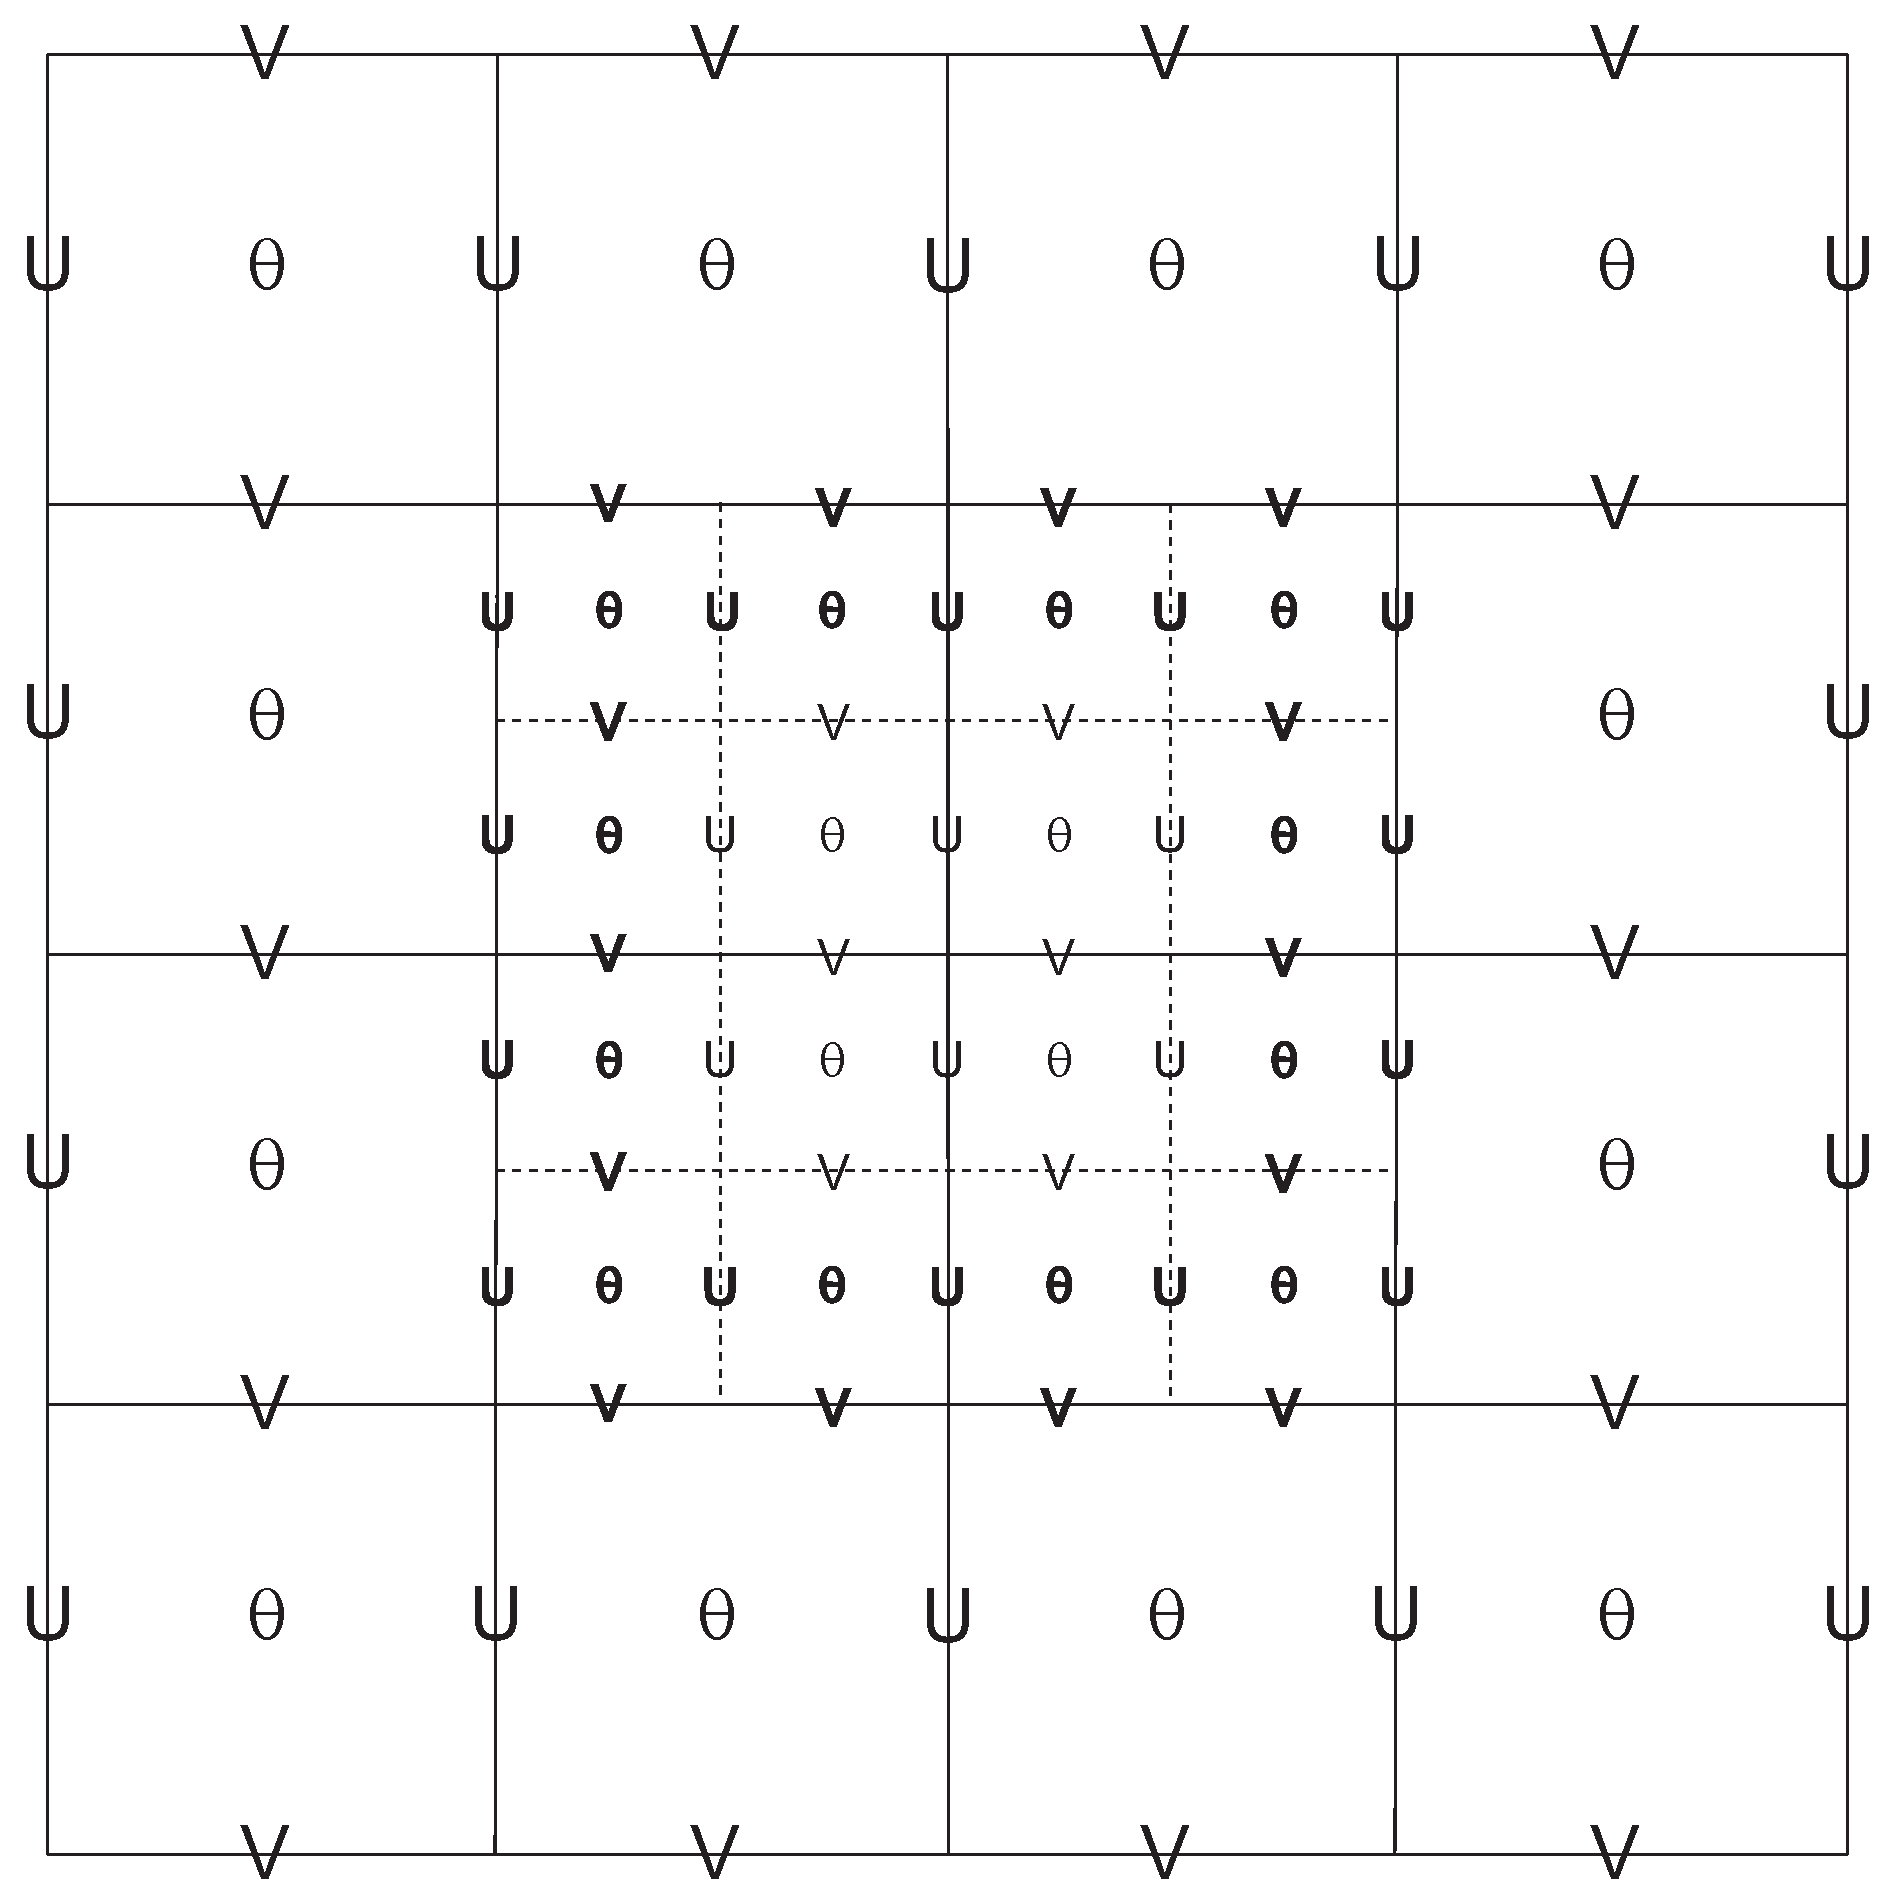
\includegraphics[width=4in]{figures/cg_fg_x2.pdf}
  \caption{\label{figure:cg_fg_x2}
Similar to Fig. \ref{figure:cg_fg}, but with a 2:1 grid-distance ratio.
}
\end{figure}

\section{Nested Lateral Boundary Conditions}
\label{nest-lbc}

For the fine grid with 2-way nesting or 1-way nesting 
(using a concurrent ARW simulation, see 
Fig. \ref{figure:12way}),
the boundary conditions are specified by the parent grid
at every coarse-grid time step. The nest lateral boundary condition behaves similarly to the 
specified boundary condition for real-data cases (see Section \ref{lbc_spec}), but
the relaxation zone is not active. Prognostic variables are entirely specified in the outer row and column
of the fine grid through spatial and temporal interpolation from the coarse grid (the coarse grid is
stepped forward in time prior to advancement of any child grid of that parent).

\section{Steps to Generate a Nest Grid}

Only the concurrent 1-way nest option or the 2-way nest
option are considered in this section.  The 1-way nest option (using two
consecutive ARW simulations, see Fig. \ref{figure:12way}) 
is functionally similar to two separate,
single-grid simulations and does not fit the following description.  For
a multiple grid simulation within a single model run, there are some
additional infrastructure steps that are required (briefly described in
Fig. \ref{nest_domain_integration_figure}).  While the following text
details a simulation with a single coarse-grid and a single fine-grid,
this implies no lack of generality when handling multiple grid levels or
multiple grids on the same level.  

\noindent
\begin{figure}[h!]  %[nest]
\setlength{\fboxrule}{.75pt}
\framebox[\columnwidth]{
\parbox{6.5truein}{
\vskip 5truept
\noindent
{\bf Integrate Parent Grid One Time Step} \medskip \hfill \break
%
\hphantom{Begin} {\bf If Nest Grid Start Time}  \smallskip \hfill \break
\hphantom{BeginBegin}
(1) Horizontally Interpolate Parent to Child Grid \hfill \break
\hphantom{BeginBegin}
(2) Optionally Input High-Resolution Child Data \hfill \break
\hphantom{BeginBegin}
(3) Compute Child Reference State \hfill \break
\hphantom{BeginBegin}
(4) Feedback Child Initial Data to Parent Grid \hfill \break
\hphantom{BeginBegin}
(5) Re-Compute Parent Reference State \hfill \break
\hphantom{Begin} {\bf End If Nest Grid Start Time}  \medskip \hfill \break
%
\hphantom{Begin} {\bf Solve Time Step for Parent Grid (see Fig. \ref{time_integration_figure})}  \medskip \hfill \break
%
\hphantom{Begin} {\bf If Nest Grid Move Time and FG Away from CG Boundary}  \smallskip \hfill \break
\hphantom{BeginBegin}
(1) Move Nest Grid (Vortex Following or Prescribed)\hfill \break
\hphantom{BeginBegin}
(2) Horizontally Translate Data Due to Grid Shift \hfill \break
\hphantom{BeginBegin}
(3) Horizontally Interpolate Parent to Child Grid (Along New Boundary) \hfill \break
\hphantom{BeginBegin}
(4) Optionally Input High-Resolution Child Topo-Landuse Data \hfill \break
\hphantom{BeginBegin}
(5) Compute Child Reference State \hfill \break
\hphantom{BeginBegin}
(6) Feedback Child Initial Data to Parent Grid \hfill \break
\hphantom{BeginBegin}
(7) Re-Compute Parent Reference State \hfill \break
\hphantom{Begin} {\bf End If Nest Grid Move Time}  \medskip \hfill \break
%
\hphantom{Begin} {\bf While Existing Nest Grids to Integrate}  \smallskip \hfill \break
\hphantom{BeginBegin}
(1) Lateral Forcing from Parent Grid to Child \hfill \break
\hphantom{BeginBegin}
(2) Integrate Child Grid to Current Time of Parent Grid\hfill \break
\hphantom{BeginBegin}
(3) Feedback Child Grid Information to Parent Grid \hfill \break
\hphantom{Begin} {\bf End While Existing Nest Grids to Integrate}  \medskip \hfill \break
%
{\bf End Grid Integrate}
\vskip 5truept
}
}
\caption{Nest grid integration sequence.}
\label{nest_domain_integration_figure}
\end{figure}

\subsubsection{Nest Instantiation}

The fine grid is instantiated as a child 
of a parent grid at the requested start time.
This initialization is within the integration step for the parent 
grid, so no child grid can begin if the parent is not active.  
To fill in the correct meteorological 
fields, an initialization routine is called to horizontally interpolate
the coarse-grid data to the fine grid locations using a monotone
interpolation scheme \citep[described in][]{smolargrell92} for most fields 
(i.e., the same scheme employed for generating the fine grid lateral
boundary conditions)
and a simple linear interpolation or averaging scheme for masked or
categorical fields.
For fields that are masked with the land/sea background (such 
as land only fields (e.g., snow), or water only fields (e.g., sea ice)), the 
interpolator needs to know what field defines the template for the masking
(such as the land use category).  Part of the automatic code generation handles
calling each field with its associated interpolator.

\subsubsection{Fine Grid Input}

After the horizontal interpolation is completed, a few orographic-based variables 
are saved so that they may be used to blend the lateral boundaries
along the coarse-grid/fine-grid interface.  
The terrain elevation, 
$\overline {\mu}_d$,
and the reference geopotential ($\overline{\phi}$) are stored for later use.
The fields selected as input from the fine grid input file (for the
concurrent 1-way and 2-way forecast methods shown in Fig. \ref{figure:12way}) are ingested, and
they overwrite the arrays that were horizontally interpolated from the
coarse grid.  No quality control for data consistency is performed
for the fine grid input.  All such masked checks are
completed by the ARW real-data pre-processor {\it real}.

\subsubsection{Interface Blended Orography}

To reduce lateral boundary noise entering the fine grid, the fine grid topography has two 
zones of smoothing, as seen in Fig. \ref{figure:12way}.
The first zone is along the outer edge of the fine domain and 
extends into the nest, with a width defined the same as the number of coarse grid points
in the width of the lateral boundary file.  In this first zone, the topography is horizontally
interpolated from the coarse grid.  The second zone extends inward from the first zone, with a
user-defined width.  The topography is linearly weighted between the interpolated coarse-grid
topography and the fine-grid topography, and it ramps from 100\% coarse-grid 
topography (at the interface between 
first and second zones) to 100\%
fine-grid topography interior to second zone.  
\noindent
The weighting scheme in the second zone (assuming a width of 5 fine-grid cells) is given as:
\begin{itemize}\setlength{\parskip}{-4pt}
\item row/column 1: 100\% interpolated coarse grid, 0\% fine grid,
\item row/column 2: 75\% interpolated coarse grid, 25\% fine grid,
\item row/column 3: 50\% interpolated coarse grid, 50\% fine grid,
\item row/column 4: 25\% interpolated coarse grid, 75\% fine grid, and
\item row/column 5: 0\% interpolated coarse grid, 100\% fine grid,
\end{itemize}
\noindent 
where row=1 is the first row in the second zone, and where the row or column 
nearest the outer edge takes precedence in ambiguous corner zones.  
The reference variables computed from the topography,
$\overline{\mu}_d$ and $\overline{\phi}$, are similarly treated.
The blended arrays are required to compute the reference state for the
fine grid.  The blending along the inner rows and columns ramps the 
coarse grid reference state to the
fine grid reference state for a smooth transition between the grids.

%
% zones of topo smoothing
%
\begin{figure} 
 \centering
  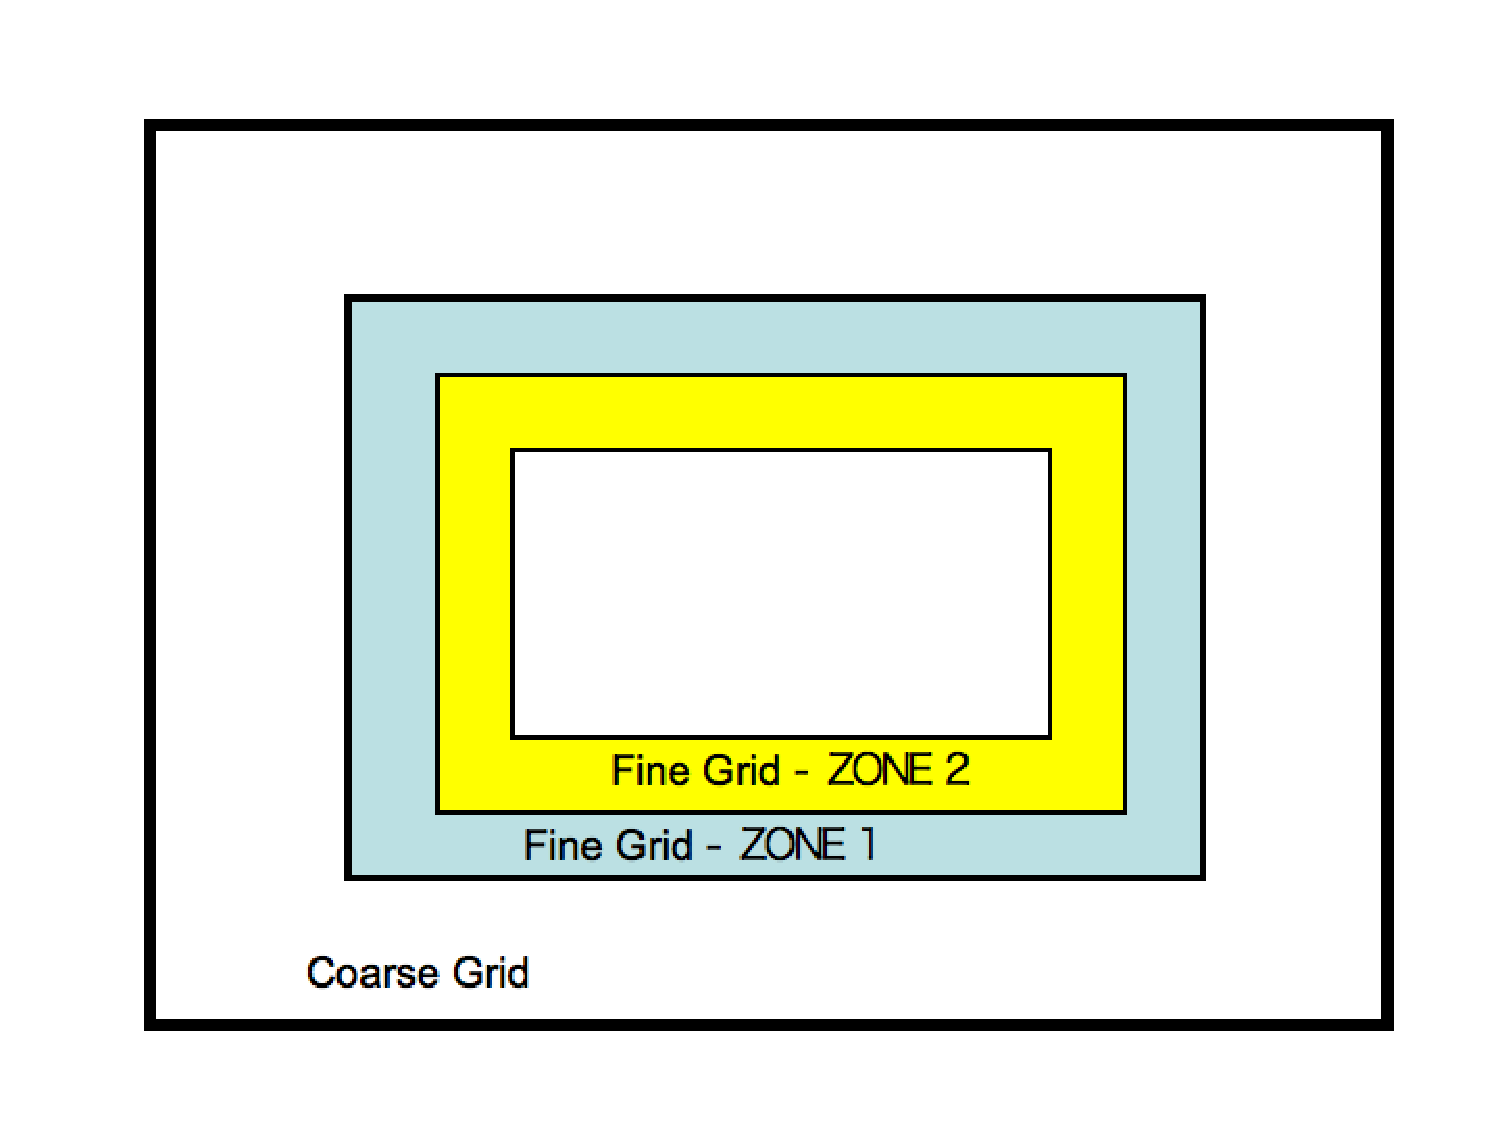
\includegraphics[width=4.5in]{figures/zone12.pdf}
  \caption{\label{figure:zone12} 
Zones of topographic blending
for a fine grid.  In the fine grid, the first zone is
entirely interpolated from the coarse grid topography.  In
the second zone, the topography is linearly weighted between
the coarse grid and the fine grid.}
\end{figure}

\subsubsection{Feedback}
So that the coarse grid and the fine grid are consistent at coincident points, the 
fine grid values are fed back to the coarse grid.
There are two available 
options for feedback: either the mean of all fine grid cells contained 
within each coarse grid cell is fed back (or cell faces in the case of the
horizontal momentum fields), or a single-point feedback 
is selected for the masked or categorical fields.

Subsequent to the feedback step, the coarse grid may be optionally smoothed in the area
of the fine grid.  Two smoothers are available: a 5-point 1-2-1 smoother and a smoother-desmoother
with a similar stencil size.
Both the feedback and the smoothers are run one row and column in from the 
interface row and column of the coarse grid that provides
the lateral boundary conditions to the fine grid.

\subsubsection{Reference State}
The initial feedback when the nest is instantiated ensures
that the coarse grid is consistent with the fine grid, particularly 
with regards to elevation and the reference state fields inside the blended region, and for such 
terrestrial features as coasts, lakes, and islands.  The adjustment 
of the elevation in the coarse grid forces a base state recalculation.  
The fine-grid needs an initial base state calculation, and after
the terrain feedback, the coarse grid is also in need of a base state
recalculation.

Note that with the horizontal interpolation of the coarse grid 
to the fine grid and the feedback of the fine grid to the coarse 
grid, 
the coarse grid base state is recomputed 
even without a separate fine-grid initial data file, 
since the coarse grid topography is adjusted.

With the completed base state computations, which follow similarly to
that described for the real-data initialization in section
\ref{initialization_real_base_section},
the routines return 
back to the integration step for the coarse and fine grids.
The fine grid data is now properly initialized for integration and
can be advanced forward a time step.

\subsubsection{Integration}

The integration by grid is recursive.  At the end of each grid's time step, a check
is made to determine if a child grid exists for that parent and if the
current time is bracketed by the child's start/end time.  
This is shown in Fig. \ref{nest_domain_integration_figure}.  The integration process for the nest (step 2 under the
while loop) is recursively calling the top step in the overall sequence as a coarse grid itself.
This is a ``depth first'' 
traversal of the tree of grids.
If a child grid does exist, that child grid is integrated up through the current time of 
the parent grid.

\subsubsection{Interpolation Options}

The parent domain (coarse grid, CG) must be interpolated to the child domain 
(fine grid, FG) prior to the CG data being used by the FG. There are several 
occurrences of this interpolation.
\begin{itemize}\setlength{\parskip}{-4pt}
\item At initialization or upon a domain move, horizontally interpolate all 
non-masked fields from CG to FG.
\item At initialization or upon a domain move, topography elevation (and 
fields derived from topography elevation) within the FG domain are blended 
with data from the CG, as shown in Fig. \ref{figure:zone12}.
\item At the completion of each CG timestep, the CG fields are interpolated
for use by the FG. Primarily, this is for the construction of the lateral boundary 
conditions for the FG domain, but optional interpolations of fields only computed 
on the most-coarse grid are available (examples include stochastic forcing and 
simple ocean models that are only defined on the outer-most domain).
\end{itemize}
\noindent 
ARW supports a number of horizontal interpolation options, available via
the user-defined namelist.
